%\documentclass{article}
\documentclass[a4paper,10pt]{article}
\renewcommand{\baselinestretch}{0.75}
\usepackage[utf8]{inputenc}
\usepackage[right=1.0cm,left=1.0cm,top=1.5cm,bottom=1.0cm]{geometry}
\usepackage{amsmath}
\usepackage{geometry}
\usepackage{parskip}
\usepackage[pdftex]{graphicx}

\usepackage[utf8]{inputenc}
%%%%%
\usepackage{secdot}
\usepackage{hyperref}
\usepackage{amsthm}
\usepackage{setspace}
\usepackage{hyperref}
\usepackage{glossaries}
\usepackage{amsmath} % For advanced math features
\usepackage{amssymb} % For \mathbb and other math symbols
%\bibliography


\doublespacing
%\pagestyle{empty}

%\geometry{a4paper, margin=1in}

\title{Solution to Question 3: Dynamic causal Bayesian optimization and optimal intervention}
\author{}
\date{}

\begin{document}

\maketitle

%\section*{Questions and Answers}
PART 1 
\subsection*{1. causal graph with 15 nodes at each time step -- 7 non-manipulable, 7 manipulable, and 1 target variable}

\textbf{Answer:} The real world example of causal graph involving 15 nodes at each step (7 non-manipulable, 7 manipulable, and 1 target variable). Imagine a scenario where the optimization of patient recovery rate in hospital setting is of utmost importance, the dynamic causal model could be used. The causal graph at each time step consists of 15 nodes: 7 non-manipulable variables (e.g., air quality, local weather, community infection rates), 7 manipulable variables (e.g., nurse-to-patient ratio, ICU bed allocation, availability of specialized doctors), and 1 target variable representing patient recovery rates. Non-manipulable variables influence both manipulable variables and recovery rates, while manipulable variables can be intervened upon to improve outcomes. Temporal dependencies between variables across time steps capture how factors evolve and affect future states. This scenario demonstrates the applicability of dynamic causal Bayesian optimization (DCBO) in designing a sequence of optimal interventions to maximize recovery rates in dynamically evolving systems while accounting for external factors~\cite{aglietti2021dynamic}. For this purpose, codes have been developed to generate the causal graph and exploration set as shown in Figure 1.  While the causal diagram is essential for understanding relationships and dependencies, it is not sufficient for deriving exploration sets or optimizing interventions. Incorporating interventional costs, constraints, and domain knowledge is crucial. Interventional costs balance target optimization with resource feasibility, while constraints address real-world limitations like resource or time restrictions. Domain knowledge refines structural equation models (SEMs) and intervention domains, ensuring alignment with practical scenerio and enhancing reliability. Programmatic generation of exploration sets adds flexibility and scalability, particularly for large or complex temporal systems, by dynamically producing subsets of manipulable variables within defined constraints. Together, these elements create a robust framework for optimizing interventions and analyzing dynamic causal systems.

The graph shown in Figure~\ref{fig:fifteen_nodes} models dependencies across time steps, connecting variables to their counterparts (e.g., $X10 \rightarrow X11 \rightarrow X12$) and linking X (manipulable) and Z (non-manipulable) variables to the target variable $(Y_t)$ at each step. It captures complex interactions where interventions on X directly and indirectly influence Y. Exploration sets are derived from subsets of X and Z based on their causal impact on Y.

\begin{figure}[h!]
 \centering
  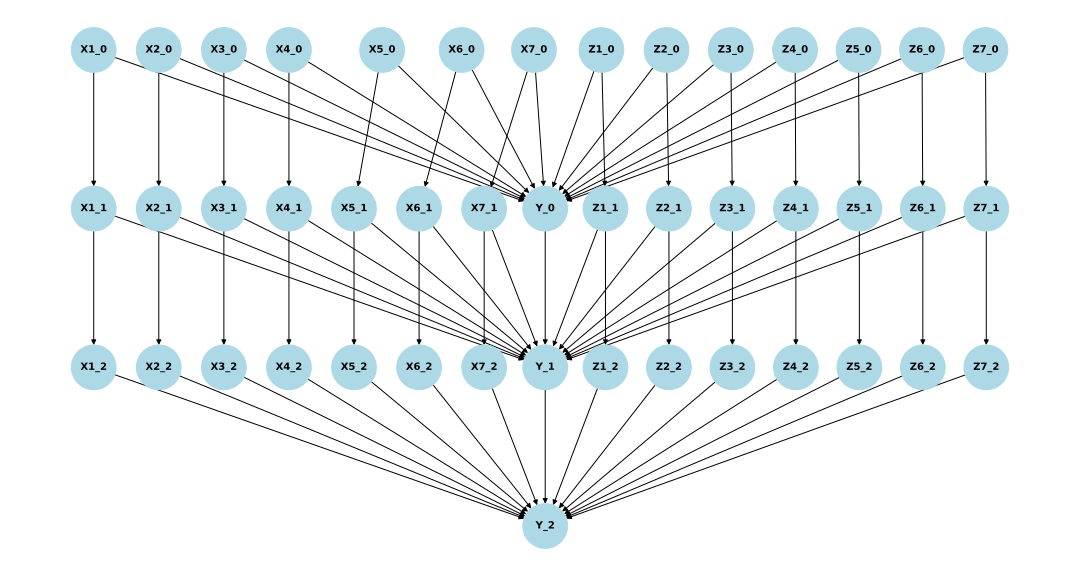
\includegraphics[width=0.9\textwidth]{fifteen_nodes_per_time_Step}
 \caption{Caussal graph with 15 nodes at each time step with 7 manipulable, 7 non-manipulable and 1 target variable}
\label{fig:fifteen_nodes}
 \end{figure}
\newpage

\subsection*{2.  Replicate their results synthetic experiments in tensorflow }

\textbf{Answer:} Please check the Jupyter notebook for the replication of their synthetic experiments using TensorFlow. The TensorFlow-based code for the causal graph (see Figure~\ref{fig:fifteen_nodes}) and its exploration set is also included. Note that the tensorflow probability aspect is still in progress.


\subsection*{3a. What are the key ideas of this paper? What are the ideas that excite you the most? Why do you find them interesting and critical?}

\textbf{Answer:} The key idea of this paper is the development of Dynamic Causal Bayesian Optimization (DCBO), a novel framework that integrates causal inference, Gaussian process modeling, and sequential decision-making to optimize interventions in dynamic systems where causal relationships evolve over time. What excites me most is the ability of DCBO to efficiently combine observational and interventional data across time steps, leveraging causal graphs to dynamically update intervention strategies. This approach is fascinating because it addresses real-world challenges in dynamic environments, such as biology and economics, where static models fail to capture temporal dependencies. By advancing optimization in causal dynamical systems, DCBO has the potential to significantly improve decision-making under uncertainty, a critical capability for applications ranging from precision medicine to resource allocation.

\subsection*{3b. Do you think the acquisition function is correct?  Is there any typo? If yes, can you explain?  If not, can you derive the correct one?}

The acquisition function proposed in the paper is defined as:

\begin{equation}
EI_{S,t}(\mathbf{x}) = \frac{\mathbb{E}_{p(y_{s,t})}[\max(y_{s,t} - y^*_t, 0)]}{\text{cost}(X_{s,t}, \mathbf{x}_{s,t})}.
\end{equation}

While this acquisition function is correct as it follows the common acquistion function used in Bayesian optimization, there are some noticeable issue that could cause potential numerical issues.  The numerator 
\(\mathbb{E}_{p(y_{s,t})}[\max(y_{s,t} - y^*_t, 0)]\) is consistent with the standard formulation of Expected Improvement (EI). It evaluates the expected gain over the current best observed value \(y^*_t\), and appears to be conceptually correct. Also, incorporating the intervention cost \(\text{cost}(X_{s,t}, \mathbf{x}_{s,t})\) in the denominator is reasonable for balancing the improvement with cost-awareness (indicating the cost of intervention). However, it should be clearly stated in the paper that there will alway be a cost of intervention, meaning that the cost of intervention should not be zero. If the cost is zero for some interventions, this would cause a division by zero. A safeguard should be implemented by adding a small positive constant \(\epsilon\) to the denominator to ensure numerical stability. Another idea is to implement the constraint acquisition function where the cost is non-zero everywhere and at every steps/stage of the opimization algorithm, and taking into consideration the cumulative system history. The following acquisition function is proposed:

\begin{equation}
EI_{S,t}(\mathbf{x}) = \frac{\mathbb{E}_{p(y_{s,t} | X_{s,t} = \mathbf{x}_{s,t}, \mathcal{H}_{0:t-1})}[\max(y_{s,t} - y^*_t, 0)]}{\max(\text{cost}(X_{s,t}, \mathbf{x}_{s,t}), \eta)},
\end{equation}

where:
\begin{itemize}
    \item \(p(y_{s,t} | X_{s,t} = \mathbf{x}_{s,t}, \mathcal{H}_{0:t-1})\) is the predicted distribution of the target \(y_{s,t}\), given the current intervention variables \(X_{s,t}\), the intervention values \(\mathbf{x}_{s,t}\), and the history \(\mathcal{H}_{0:t-1}\), which includes all past interventions and observations. 
    \item \(\mathcal{H}_{0:t-1}\) represents the cumulative system history at time \(t\). This clearly incorporating causal priors and past interventions into \(p(y_{s,t})\).
    \item \(\text{cost}(X_{s,t}, \mathbf{x}_{s,t}) > 0\) is the intervention cost for the variable set \(X_{s,t}\) at the given values \(\mathbf{x}_{s,t}\).
    \item \(\eta > 0\) is a small positive threshold ensuring that the denominator is bounded below by \(\eta\), preventing the cost from becoming too small.
\end{itemize}
   

\subsection*{3c. Do you find any errors or questionable issues? }

The assumption that the causal graph  $G(t)$ remains invariant across all time steps ($G(t) = G(0) \rm\, for \,all \,t>0$) simplifies modeling but overlooks real-world scenarios where causal relationships evolve dynamically, as seen in biological or economic systems. Similarly, the exploration set ${P(X_{t})}$, derived from the power set of manipulable variables ${X}_{t}$, grows exponentially with the number of variables, and while assumed constant over time, its scalability in larger systems remains a challenge. Additionally, the acquisition function, while incorporating intervention costs, may overly favor low but nonzero costs, potentially leading to suboptimal decisions; introducing a minimum cost threshold could mitigate this issue. The additive assumption for $Y_t$ (i.e., $Y_t = f_Y(Pa(Y_t)) + \epsilon$) may oversimplify complex, non-additive causal relationships often found in real-world systems. Finally, while the integration of observational and interventional data is a strength, the paper does not address inconsistencies or noise between these data types, which could compromise the model's accuracy, highlighting the need for mitigation strategies. Lastly, this paper assumes additive white noise, could other noise model be used? what is the implication of using different noise models and varying noise levels? Could this significantly affect the model performance? All these questions are either not clearly shown or remain largely unanswered in the paper. 



\subsection*{3d. Are there any parts that are not clear in the paper?}

\textbf{Answer:} There are inconsistencies in the theory, and the notation is hard to follow in some parts of the paper. I believe all symbols, notations and abrreviation used in the paper should be clearly defined in the tagged-A supplementary information. Many notations/symbols are not included in the nomenclature (to mention few, no any list of abbreviations, and $C, \mathbf{F}, \mathbf{C}$, noise variable $\epsilon$ etc., are not included). The explanation of the assumption that the causal graph $G(t)$ remains invariant over time is unclear, especially regarding its implications for dynamic systems. The investigation of different noise levels and their effect on the integration of observational and interventional data is insufficiently detailed. Additionally, the exponential growth of the exploration set $P(X_t)$ with the number of manipulable variables poses scalability challenges, which are not adequately addressed in the context of larger systems. Lastly, the derivation and justification of the acquisition function $EI_{S,t}(x)$ , particularly its dependence on cost, lacks clarity, especially in scenarios where intervention costs are small or unevenly distributed.

\subsection*{3e. Can you please include derivations that are not clear in their paper?}


\textbf{Answer:} The proof of theorem 1 and derivation of DAG1 and 2 in supplementary material are not clearly presented. More details can be added to enable better understanding of the paper. The drivation of $\mathbb{E}[Y_1 \mid do(Z_1 = z), I_0]$, $\mathbb{E}[Y_1 \mid do(X_1 = x), I_0]$, $\mathbb{E}[Y_2 \mid do(X_2 = x_2), I_0, I_1]$, $\mathbb{E}[Y_2 \mid do(Z_2 = z_2), I_0, I_1]$ etc, can be more clearly expressed. The following shows clear step-by-step derivation of $\mathbb{E}[Y_1 \mid do(Z_1 = z), I_0]$ to enrich reader's understanding:

To compute the expectation \(\mathbb{E}[Y_1 \mid do(Z_1 = z), I_0]\), we start with the definition of conditional expectation:
\[
\mathbb{E}[Y_1 \mid do(Z_1 = z), I_0] = \int y_1 p(y_1 \mid do(Z_1 = z), I_0) \, dy_1.
\]

Using the joint probability distribution of \(Y_1\) and \(Y_0\), the parent of \(Y_1\), we rewrite the expression as:
\[
\mathbb{E}[Y_1 \mid do(Z_1 = z), I_0] = \int \int y_1 p(y_1 \mid y_0, do(Z_1 = z), I_0) p(y_0 \mid do(Z_1 = z), I_0) \, dy_1 \, dy_0.
\]

The structural equation for \(Y_1\) is given by:
\[
Y_1 = f_Y^Y(Y_0) + f_Y^{NY}(Z_1) + \epsilon_Y,
\]
where \(f_Y^Y(Y_0)\) represents the contribution of \(Y_0\), \(f_Y^{NY}(Z_1)\) is the non-target causal effect of \(Z_1\), and \(\epsilon_Y\) is the noise term. Based on this structural equation, the conditional probability \(p(y_1 \mid y_0, do(Z_1 = z), I_0)\) can be expressed as:
\[
p(y_1 \mid y_0, do(Z_1 = z), I_0) = \delta(y_1 - [f_Y^Y(y_0) + f_Y^{NY}(z)]),
\]
where \(\delta(\cdot)\) is the Dirac delta function, representing a deterministic relationship.

Substituting this into the integral, we have:
\[
\mathbb{E}[Y_1 \mid do(Z_1 = z), I_0] = \int \int y_1 \delta(y_1 - [f_Y^Y(y_0) + f_Y^{NY}(z)]) p(y_0 \mid do(Z_1 = z), I_0) \, dy_1 \, dy_0.
\]

The delta function forces \(y_1 = f_Y^Y(y_0) + f_Y^{NY}(z)\). This simplifies the inner integral:
\[
\int y_1 \delta(y_1 - [f_Y^Y(y_0) + f_Y^{NY}(z)]) \, dy_1 = f_Y^Y(y_0) + f_Y^{NY}(z).
\]

Thus, the expectation becomes:
\[
\mathbb{E}[Y_1 \mid do(Z_1 = z), I_0] = \int \big(f_Y^Y(y_0) + f_Y^{NY}(z)\big) p(y_0 \mid do(Z_1 = z), I_0) \, dy_0.
\]

Expanding the integral, we separate the terms:
\[
\mathbb{E}[Y_1 \mid do(Z_1 = z), I_0] = \int f_Y^Y(y_0) p(y_0 \mid do(Z_1 = z), I_0) \, dy_0 + f_Y^{NY}(z) \int p(y_0 \mid do(Z_1 = z), I_0) \, dy_0.
\]

The second integral represents the normalization of \(p(y_0 \mid do(Z_1 = z), I_0)\), which equals 1. Therefore:
\[
\mathbb{E}[Y_1 \mid do(Z_1 = z), I_0] = \int f_Y^Y(y_0) p(y_0 \mid do(Z_1 = z), I_0) \, dy_0 + f_Y^{NY}(z).
\]

The first term represents the contribution of the past target variable \(Y_0\). Denoting the expected value of \(Y_0\) under the intervention by \(y_0^\ast\), this term simplifies to:
\[
\int f_Y^Y(y_0) p(y_0 \mid do(Z_1 = z), I_0) \, dy_0 = f_Y^Y(y_0^\ast).
\]

Finally, the expression for \(\mathbb{E}[Y_1 \mid do(Z_1 = z), I_0]\) becomes:
\[
\mathbb{E}[Y_1 \mid do(Z_1 = z), I_0] = f_Y^Y(y_0^\ast) + f_Y^{NY}(z).
\]

Here:
\begin{itemize}
    \item \(f_Y^Y(y_0^\ast)\): Represents the contribution of the past target \(Y_0\).
    \item \(f_Y^{NY}(z)\): Captures the direct non-target causal effect of \(Z_1\).
\end{itemize}

\subsection*{3f. Is there any important part of their code that is not mentioned in the paper?}

\textbf{Answer:} Yes, there are good illustrative examples where the optimal outcomes obtained from Causal Bayesian Optimization (CBO)~\cite{aglietti2020causal}, Bayesian Optimization (BO)~\cite{nyikosa2018bayesian}, Adaptive Bayesian Optimization (ABO)~\cite{nyikosa2018bayesian}, and DCBO are compared against the ground truth. While these comparisons are insightful as demonstrated in the paper and their code, none of these plots/results are reported in the paper.


\subsection*{3g Can you explain the paper based on details you have learnt from their code and your result replication experience?}

\textbf{Answer:} The paper on Dynamic Causal Bayesian Optimization (DCBO)~\cite{aglietti2021dynamic} presents a novel methodology for optimizing interventions in dynamic systems by integrating causal inference and Bayesian optimization frameworks. Through replication of their results, I gained a deeper understanding of how the proposed approach operates. The key innovation lies in its ability to model both temporal dependencies and causal relationships using a combination of static and dynamic Structural Equation Models (SEMs), supported by Gaussian Processes (GPs) as surrogate models. The implementation involves constructing dynamic causal graphs, creating exploration sets, and leveraging emission and transition functions to estimate intervention effects over time. The code demonstrates the utility of DCBO in efficiently optimizing interventions by recursively updating the surrogate model and computing the acquisition function over a multi-dimensional intervention grid. Visualizations from the replication experiments confirm that DCBO outperforms competing methods like CBO, ABO, and BO, particularly in dynamic scenarios where temporal dependencies play a significant role. These results validate the theoretical claims in the paper, showcasing the robustness of DCBO in identifying cost-effective and optimal interventions while accounting for causal structures and system dynamics.

\subsection*{3h. Can you think of a possible application of such techniques for a bank?}


\textbf{Answer:} DCBO offers a powerful decion-making framework for addressing complex challenges in the banking sector, particularly in dynamic loan portfolio management. By modeling causal relationships between macroeconomic factors (e.g., GDP growth, unemployment rates), customer-specific variables (e.g., credit scores, income), and loan outcomes (e.g., repayment probability, default risk), DCBO enables banks to optimize interventions over time. Using Structural Equation Models (SEMs), the approach captures both immediate effects of variables (through emission functions) and their temporal dependencies (via transition functions). For instance, banks can use DCBO to dynamically adjust loan terms, such as interest rates or credit limits, in response to changing economic conditions or evolving customer risk profiles. Additionally, it can guide decisions about offering targeted refinancing options or rebalancing loan portfolios to minimize risk and maximize profitability. The DCBO's capability to account for dynamic changes, causal complexity, and cost-effectiveness makes it an ideal tool for improving loan repayment rates, managing portfolio risk, and enhancing overall financial performance in a dynamic and uncertain banking environment.

\newpage
PART 2

\subsection*{a.}



\clearpage
%\bibliographystyle{plain}
\bibliographystyle{plain} % Specify the bibliography style
\bibliography{myref}


\end{document}


